\documentclass[aspectratio=169]{beamer}
\usepackage{booktabs}
\usepackage{pgfplots}
\pgfplotsset{compat=1.18}
\usepackage{tikz}
\usetikzlibrary{shapes.geometric,arrows.meta,positioning,fit,backgrounds,calc,decorations.pathreplacing}
\usepackage{xcolor}
\usepackage{colortbl}
\usepackage{multirow}
\usepackage{array}
\usepackage{amsmath}

\definecolor{ADIBlue}{RGB}{0,100,175}
\definecolor{ADIRed}{RGB}{200,16,46}
\definecolor{ADIGray}{RGB}{100,100,100}
\definecolor{ADIGold}{RGB}{255,180,0}
\definecolor{LightBlue}{RGB}{230,242,255}
\definecolor{AccentGreen}{RGB}{0,150,80}
\definecolor{DarkGray}{RGB}{50,50,50}

\usetheme{Madrid}
\usecolortheme[named=ADIBlue]{structure}
\setbeamercolor{title}{fg=white,bg=ADIBlue}
\setbeamercolor{frametitle}{fg=white,bg=ADIBlue}
\setbeamercolor{block title}{fg=white,bg=ADIBlue}
\setbeamercolor{block title alerted}{fg=white,bg=ADIRed}
\setbeamerfont{title}{size=\Large,series=\bfseries}
\setbeamerfont{frametitle}{size=\normalsize,series=\bfseries}
\setbeamertemplate{navigation symbols}{}
\setbeamertemplate{footline}[frame number]

\title{ADI AI8X}
\subtitle{Hardware Products \& Model Zoo Fit Analysis}
\author{Edge AI Platform Evaluation}
\date{August 2026}
\institute{Analog Devices, Inc.}

\begin{document}

\begin{frame}\titlepage\end{frame}
\begin{frame}{Agenda}\tableofcontents\end{frame}

\section{ADI AI8X Product Portfolio}

\begin{frame}{ADI Edge AI Hardware Family}
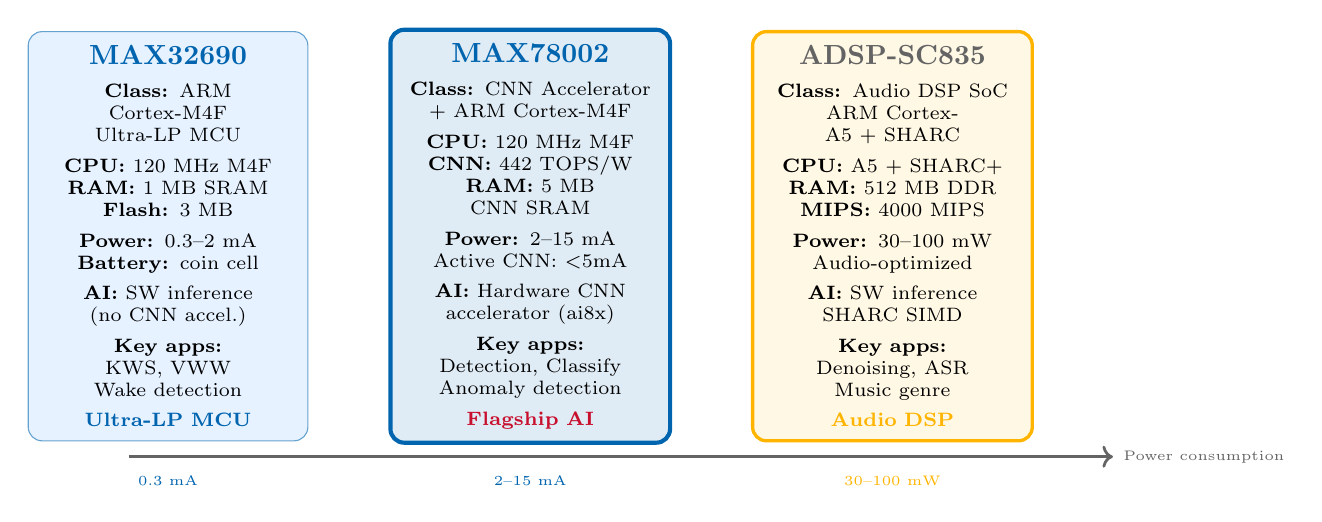
\begin{tikzpicture}[
  dev/.style={rounded corners=5pt,minimum width=3.4cm,
              minimum height=5.0cm,text width=3.2cm,align=center,
              font=\scriptsize,inner sep=5pt},
]
% MAX32690 --- ultra-low power MCU
\node[dev,draw=ADIBlue!60,fill=LightBlue] (m32) at (0,0) {
  \textcolor{ADIBlue}{\textbf{\normalsize MAX32690}}\\[4pt]
  \textbf{Class:} ARM Cortex-M4F\\Ultra-LP MCU\\[3pt]
  \textbf{CPU:} 120 MHz M4F\\
  \textbf{RAM:} 1 MB SRAM\\
  \textbf{Flash:} 3 MB\\[3pt]
  \textbf{Power:} 0.3--2 mA\\
  \textbf{Battery:} coin cell\\[3pt]
  \textbf{AI:} SW inference\\
  (no CNN accel.)\\[3pt]
  \textbf{Key apps:}\\
  KWS, VWW\\Wake detection\\[3pt]
  \textcolor{ADIBlue}{\textbf{Ultra-LP MCU}}
};
% MAX78002 --- CNN accelerator
\node[dev,draw=ADIBlue,fill=ADIBlue!12,line width=1.5pt] (m78) at (4.6,0) {
  \textcolor{ADIBlue}{\textbf{\normalsize MAX78002}}\\[4pt]
  \textbf{Class:} CNN Accelerator\\+ ARM Cortex-M4F\\[3pt]
  \textbf{CPU:} 120 MHz M4F\\
  \textbf{CNN:} 442 TOPS/W\\
  \textbf{RAM:} 5 MB CNN SRAM\\[3pt]
  \textbf{Power:} 2--15 mA\\
  Active CNN: $<$5mA\\[3pt]
  \textbf{AI:} Hardware CNN\\
  accelerator (ai8x)\\[3pt]
  \textbf{Key apps:}\\
  Detection, Classify\\
  Anomaly detection\\[3pt]
  \textcolor{ADIRed}{\textbf{Flagship AI}}
};
% ADSP-SC835 --- DSP SoC
\node[dev,draw=ADIGold,fill=ADIGold!10,line width=1.2pt] (sc835) at (9.2,0) {
  \textcolor{ADIGray}{\textbf{\normalsize ADSP-SC835}}\\[4pt]
  \textbf{Class:} Audio DSP SoC\\ARM Cortex-A5 + SHARC\\[3pt]
  \textbf{CPU:} A5 + SHARC+\\
  \textbf{RAM:} 512 MB DDR\\
  \textbf{MIPS:} 4000 MIPS\\[3pt]
  \textbf{Power:} 30--100 mW\\
  Audio-optimized\\[3pt]
  \textbf{AI:} SW inference\\
  SHARC SIMD\\[3pt]
  \textbf{Key apps:}\\
  Denoising, ASR\\
  Music genre\\[3pt]
  \textcolor{ADIGold}{\textbf{Audio DSP}}
};
% Power axis
\draw[->,ADIGray,line width=1pt] (-0.5,-2.8) -- (12,-2.8)
  node[right,font=\tiny]{Power consumption};
\node[font=\tiny,text=ADIBlue] at (0,-3.1) {0.3 mA};
\node[font=\tiny,text=ADIBlue] at (4.6,-3.1) {2--15 mA};
\node[font=\tiny,text=ADIGold] at (9.2,-3.1) {30--100 mW};
\end{tikzpicture}
\end{frame}

\begin{frame}{ADI Edge AI Device Specifications}
\small
\begin{tabular}{lccc}
\toprule
\textbf{Specification} & \textbf{MAX32690} & \textbf{MAX78002} & \textbf{ADSP-SC835}\\
\midrule
\textbf{Primary CPU} & ARM Cortex-M4F & ARM Cortex-M4F & ARM Cortex-A5\\
\textbf{Secondary CPU} & --- & --- & SHARC+ DSP\\
\textbf{Clock Speed} & 120 MHz & 120 MHz & 1 GHz (A5)\\
\textbf{AI Accelerator} & None & CNN HW Accel & SHARC SIMD\\
\textbf{AI Efficiency} & SW only & \textbf{442 TOPS/W} & $\sim$4 GOPS\\
\textbf{SRAM} & 1 MB & 5 MB (CNN) & 512 MB DDR\\
\textbf{Flash/Storage} & 3 MB & 16 MB & SD/eMMC\\
\textbf{Active Power} & 0.3--2 mA & 2--15 mA & 30--100 mW\\
\textbf{Sleep Power} & $<$10 $\mu$A & $<$50 $\mu$A & ---\\
\textbf{Battery life} & Years (coin) & Months & N/A\\
\textbf{Quant.\ method} & INT8 SW & INT4/INT8 HW & INT8 SW\\
\textbf{Package} & 9$\times$9 mm WLP & 9$\times$9 mm WLP & BGA\\
\textbf{Target domain} & Wearable, IoT & IoT, Industrial & Industrial audio\\
\midrule
\textbf{Model zoo models} & 5 & 8 & 4\\
\bottomrule
\end{tabular}
\end{frame}

\begin{frame}{MAX78002 CNN Accelerator Architecture}
\begin{columns}
\column{0.55\textwidth}
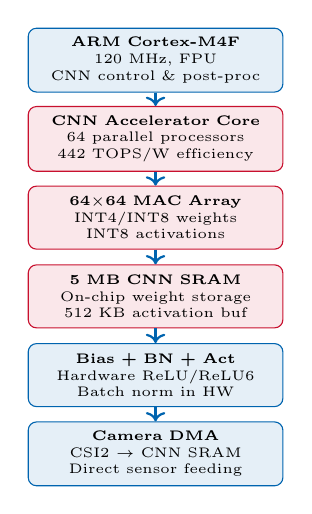
\begin{tikzpicture}[
  blk/.style={draw=ADIBlue,fill=ADIBlue!10,rounded corners=3pt,
              minimum height=0.8cm,text width=3.0cm,align=center,font=\tiny},
  ablk/.style={draw=ADIRed,fill=ADIRed!10,rounded corners=3pt,
               minimum height=0.8cm,text width=3.0cm,align=center,font=\tiny},
]
\node[blk] (cpu) at (0,5.0) {\textbf{ARM Cortex-M4F}\\120 MHz, FPU\\CNN control \& post-proc};
\node[ablk] (cnn) at (0,4.0) {\textbf{CNN Accelerator Core}\\64 parallel processors\\442 TOPS/W efficiency};
\node[ablk] (mac) at (0,3.0) {\textbf{64$\times$64 MAC Array}\\INT4/INT8 weights\\INT8 activations};
\node[ablk] (sram) at (0,2.0) {\textbf{5 MB CNN SRAM}\\On-chip weight storage\\512 KB activation buf};
\node[blk] (bias) at (0,1.0) {\textbf{Bias + BN + Act}\\Hardware ReLU/ReLU6\\Batch norm in HW};
\node[blk] (dma) at (0,0.0) {\textbf{Camera DMA}\\CSI2 $\rightarrow$ CNN SRAM\\Direct sensor feeding};
\foreach \a/\b in {cpu/cnn,cnn/mac,mac/sram,sram/bias,bias/dma}
  \draw[->,ADIBlue,line width=0.8pt] (\a) -- (\b);
\end{tikzpicture}
\column{0.42\textwidth}
\footnotesize
\begin{block}{CNN Accelerator Facts}
\begin{itemize}
  \item \textbf{64 parallel CNN processors}
  \item \textbf{INT4 weights}: halves memory vs INT8
  \item \textbf{5 MB on-chip SRAM}: entire model fits in SRAM --- no external DDR during inference
  \item \textbf{Layer fusion}: Conv+BN+Act in single pass
  \item \textbf{Zero DRAM access} during CNN inference
\end{itemize}
\end{block}
\begin{alertblock}{Why 442 TOPS/W?}
\footnotesize All weights + activations stay in on-chip SRAM. Eliminates DDR power (typically 40--60\% of inference energy in external-memory devices).
\end{alertblock}
\end{columns}
\end{frame}

\section{QAT Software Stack}

\begin{frame}{ai8x QAT Training \& Synthesis Flow}
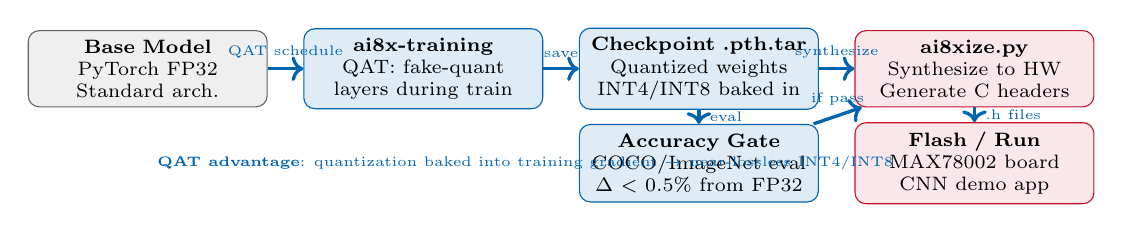
\begin{tikzpicture}[
  box/.style={rounded corners=4pt,minimum height=0.85cm,
              text width=2.8cm,align=center,font=\scriptsize},
  arr/.style={->,line width=1.2pt,ADIBlue},
]
\node[draw=ADIGray,fill=ADIGray!10,box] (base) at (0,3.0)
  {\textbf{Base Model}\\PyTorch FP32\\Standard arch.};
\node[draw=ADIBlue,fill=ADIBlue!12,box] (qat) at (3.5,3.0)
  {\textbf{ai8x-training}\\QAT: fake-quant\\layers during train};
\node[draw=ADIBlue,fill=ADIBlue!12,box] (ckpt) at (7.0,3.0)
  {\textbf{Checkpoint .pth.tar}\\Quantized weights\\INT4/INT8 baked in};
\node[draw=ADIRed,fill=ADIRed!10,box] (ai8xize) at (10.5,3.0)
  {\textbf{ai8xize.py}\\Synthesize to HW\\Generate C headers};
\node[draw=ADIRed,fill=ADIRed!10,box] (flash) at (10.5,1.8)
  {\textbf{Flash / Run}\\MAX78002 board\\CNN demo app};
\node[draw=ADIBlue,fill=ADIBlue!12,box] (eval) at (7.0,1.8)
  {\textbf{Accuracy Gate}\\COCO/ImageNet eval\\$\Delta < 0.5\%$ from FP32};
\draw[arr] (base) -- (qat) node[midway,above,font=\tiny]{QAT schedule};
\draw[arr] (qat) -- (ckpt) node[midway,above,font=\tiny]{save};
\draw[arr] (ckpt) -- (ai8xize) node[midway,above,font=\tiny]{synthesize};
\draw[arr] (ai8xize) -- (flash) node[midway,right,font=\tiny]{.h files};
\draw[arr] (ckpt) -- (eval) node[midway,right,font=\tiny]{eval};
\draw[arr] (eval) -- (ai8xize) node[midway,above,font=\tiny]{if pass};
\node[font=\tiny,text=ADIBlue,anchor=west] at (0,1.8)
  {\textbf{QAT advantage}: quantization baked into training gradient $\rightarrow$ near-lossless INT4/INT8};
\end{tikzpicture}
\end{frame}

\begin{frame}{QAT vs PTQ: Why ADI Chose QAT}
\begin{columns}
\column{0.52\textwidth}
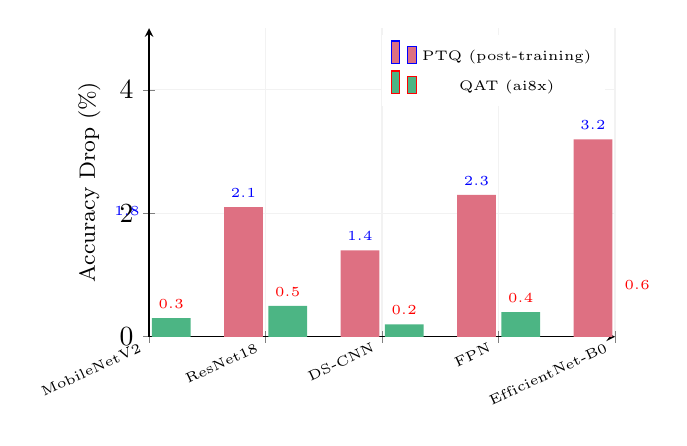
\begin{tikzpicture}
\begin{axis}[
  ybar,
  width=7.5cm,height=5.5cm,
  bar width=14pt,
  ylabel={\footnotesize Accuracy Drop (\%)},
  xtick=data,
  xticklabels={MobileNetV2,ResNet18,DS-CNN,FPN,EfficientNet-B0},
  xticklabel style={font=\tiny,rotate=25,anchor=east},
  ymin=0,ymax=5,
  grid=major,grid style={gray!10},
  axis lines=left,
  legend style={font=\tiny,at={(0.98,0.98)},anchor=north east,draw=none},
  nodes near coords,nodes near coords style={font=\tiny},
]
\addplot+[fill=ADIRed!60,draw=none]
  coordinates {(0,1.8)(1,2.1)(2,1.4)(3,2.3)(4,3.2)};
\addlegendentry{PTQ (post-training)}
\addplot+[fill=AccentGreen!70,draw=none]
  coordinates {(0,0.3)(1,0.5)(2,0.2)(3,0.4)(4,0.6)};
\addlegendentry{QAT (ai8x)}
\end{axis}
\end{tikzpicture}
\column{0.45\textwidth}
\footnotesize
\begin{block}{QAT Benefits for MAX78002}
\begin{itemize}
  \item \textbf{$<$0.6\%} accuracy drop across all models (vs 1.4--3.2\% PTQ)
  \item Gradients flow through fake-quant nodes --- model \emph{learns} to be quantization-robust
  \item INT4 weights supported (impossible with PTQ)
  \item Matches MAX78002 hardware precision exactly during training
\end{itemize}
\end{block}
\begin{alertblock}{Critical: op-set constraint}
\footnotesize MAX78002 CNN accel supports only specific ops. Models must be designed for this op-set --- QAT training enforces it.
\end{alertblock}
\end{columns}
\end{frame}

\section{Model Zoo: Vision Models}

\begin{frame}{Vision Models --- Device Fit Analysis}
\small
\begin{tabular}{lcccl}
\toprule
\textbf{Model} & \textbf{Metric} & \textbf{Device} & \textbf{Latency} & \textbf{Why fits}\\
\midrule
\multicolumn{5}{l}{\textit{Classification --- MAX78002}}\\
mobilenetv2\_050 & 62.0\% & MAX78002 & $\sim$3ms & INT4 wts, 1.4M params fit 5MB CNN SRAM\\
mobilenetv2\_075 & 65.0\% & MAX78002 & $\sim$5ms & 2.6M params, 2$\times$ INT4 weight saving\\
simplenet & 60.0\% & MAX78002 & $\sim$2ms & Custom tiny arch for MAX78002 op-set\\
\midrule
\multicolumn{5}{l}{\textit{Classification --- MAX32690}}\\
micronet\_m & 61.5\% & MAX32690 & $\sim$20ms & Only 0.3M params; SW inference, 1MB SRAM\\
micronet\_s & 57.0\% & MAX32690 & $\sim$15ms & Smallest model: 0.2M params, 120MHz M4F\\
\midrule
\multicolumn{5}{l}{\textit{Detection --- MAX78002}}\\
feature\_pyramid\_net & 50.5\% mAP & MAX78002 & $\sim$20ms & VOC 21-class; FPN layers on CNN accel\\
tinierssd & 89.9\% (kpts) & MAX78002 & $\sim$8ms & QR keypoint task; ultra-compact head\\
\midrule
\multicolumn{5}{l}{\textit{Anomaly --- MAX78002}}\\
autoencoder\_vibration & 96.2\% AUC & MAX78002 & $\sim$5ms & 1D conv mapped to 2D MAC array\\
\bottomrule
\end{tabular}
\end{frame}

\begin{frame}{Why FPN Fits MAX78002: Layer-by-Layer Analysis}
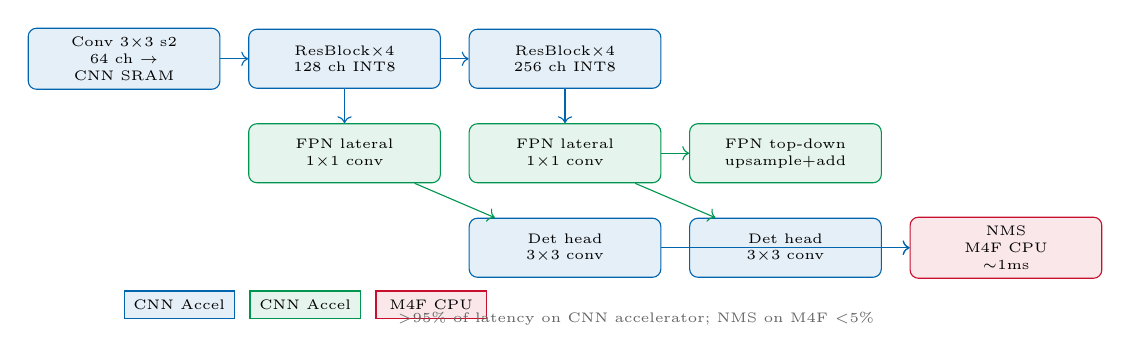
\begin{tikzpicture}[
  blk/.style={draw=ADIBlue,fill=ADIBlue!10,rounded corners=3pt,
              minimum height=0.75cm,text width=2.2cm,align=center,font=\tiny},
  cblk/.style={draw=AccentGreen,fill=AccentGreen!10,rounded corners=3pt,
               minimum height=0.75cm,text width=2.2cm,align=center,font=\tiny},
  xblk/.style={draw=ADIRed,fill=ADIRed!10,rounded corners=3pt,
               minimum height=0.75cm,text width=2.2cm,align=center,font=\tiny},
]
\node[blk] (b1) at (0,3.0) {Conv 3$\times$3 s2\\64 ch $\rightarrow$ CNN SRAM};
\node[blk] (b2) at (2.8,3.0) {ResBlock$\times$4\\128 ch INT8};
\node[blk] (b3) at (5.6,3.0) {ResBlock$\times$4\\256 ch INT8};
\node[cblk] (fpn1) at (2.8,1.8) {FPN lateral\\1$\times$1 conv};
\node[cblk] (fpn2) at (5.6,1.8) {FPN lateral\\1$\times$1 conv};
\node[cblk] (fpn3) at (8.4,1.8) {FPN top-down\\upsample+add};
\node[blk] (h1) at (5.6,0.6) {Det head\\3$\times$3 conv};
\node[blk] (h2) at (8.4,0.6) {Det head\\3$\times$3 conv};
\node[xblk] (nms) at (11.2,0.6) {NMS\\M4F CPU\\$\sim$1ms};
\draw[->,ADIBlue] (b1) -- (b2);
\draw[->,ADIBlue] (b2) -- (b3);
\draw[->,ADIBlue] (b2) -- (fpn1);
\draw[->,ADIBlue] (b3) -- (fpn2);
\draw[->,AccentGreen] (fpn1) -- (h1);
\draw[->,AccentGreen] (fpn2) -- (h2);
\draw[->,AccentGreen] (fpn2) -- (fpn3);
\draw[->,ADIBlue] (h1) -- (nms);
\draw[->,ADIBlue] (h2) -- (nms);
\draw[fill=ADIBlue!10,draw=ADIBlue] (0,-0.3) rectangle (1.4,0.05)
  node[midway,font=\tiny]{CNN Accel};
\draw[fill=AccentGreen!10,draw=AccentGreen] (1.6,-0.3) rectangle (3.0,0.05)
  node[midway,font=\tiny]{CNN Accel};
\draw[fill=ADIRed!10,draw=ADIRed] (3.2,-0.3) rectangle (4.6,0.05)
  node[midway,font=\tiny]{M4F CPU};
\node[font=\tiny,text=ADIGray] at (6.5,-0.3)
  {$>$95\% of latency on CNN accelerator; NMS on M4F $<$5\%};
\end{tikzpicture}
\end{frame}

\section{Model Zoo: Audio Models}

\begin{frame}{Audio Models --- Device Fit \& Performance}
\begin{columns}
\column{0.52\textwidth}
\small
\begin{tabular}{lccl}
\toprule
\textbf{Model} & \textbf{Acc/Score} & \textbf{Device} & \textbf{Task}\\
\midrule
ds\_cnn & 94.5\% & MAX32690 & KWS (35 keywords)\\
conv1d\_audionet & 86.3\% & MAX78002 & KWS (10 keywords)\\
rnnoise & PESQ 2.95 & ADSP-SC835 & Speech denoising\\
dtln & PESQ 2.95 & ADSP-SC835 & Music denoising\\
genrenet & 84.5\% & ADSP-SC835 & Music genre\\
\midrule
\textit{Special:} & & &\\
micronet\_vww & 76.8\% & MAX32690 & Visual wake word\\
\bottomrule
\end{tabular}
\vspace{0.4cm}
\footnotesize
\begin{block}{DS-CNN on MAX32690}
\begin{itemize}
  \item 4-layer depthwise separable CNN
  \item 40 MFCC features $\times$ 49 time frames
  \item 120 MHz M4F fully handles inference
  \item \textbf{94.5\%} on Google Speech Commands
  \item Power: $<$1 mA during inference
\end{itemize}
\end{block}
\column{0.45\textwidth}
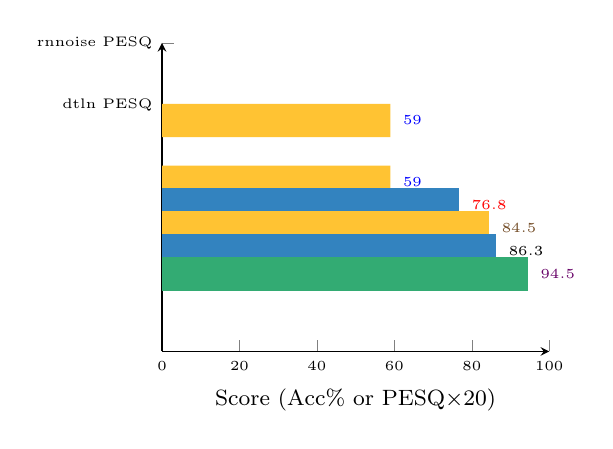
\begin{tikzpicture}
\begin{axis}[
  xbar,
  width=6.5cm, height=5.5cm,
  bar width=12pt,
  xlabel={\footnotesize Score (Acc\% or PESQ$\times$20)},
  ytick=data,
  yticklabels={rnnoise PESQ,dtln PESQ,micronet vww,genrenet,conv1d kws,ds\_cnn kws},
  yticklabel style={font=\tiny},
  xticklabel style={font=\tiny},
  xmin=0,xmax=100,
  nodes near coords,nodes near coords style={font=\tiny,xshift=1pt},
  axis lines=left,tick align=inside,
]
\addplot+[xbar,fill=ADIGold!80,draw=none] coordinates {(59,5)(59,4)};
\addplot+[xbar,fill=ADIBlue!80,draw=none] coordinates {(76.8,3)};
\addplot+[xbar,fill=ADIGold!80,draw=none] coordinates {(84.5,2)};
\addplot+[xbar,fill=ADIBlue!80,draw=none] coordinates {(86.3,1)};
\addplot+[xbar,fill=AccentGreen!80,draw=none] coordinates {(94.5,0)};
\end{axis}
\end{tikzpicture}
\end{columns}
\end{frame}

\begin{frame}{Dual Audio Routing: ADSP-SC835 Pipeline}
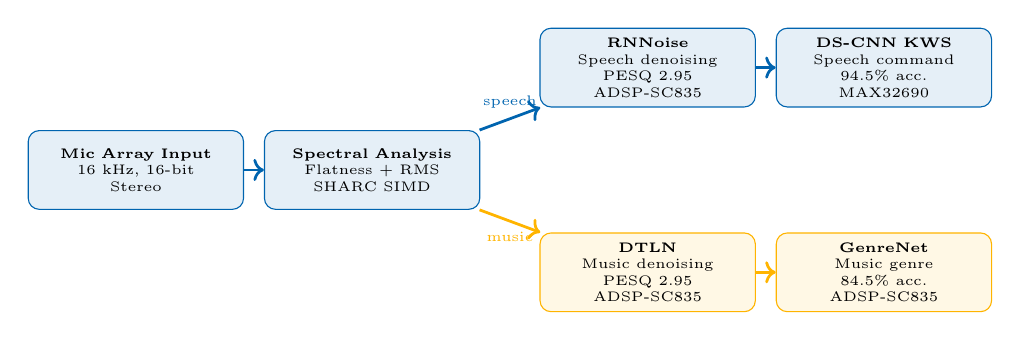
\begin{tikzpicture}[
  box/.style={draw=ADIBlue,fill=ADIBlue!10,rounded corners=4pt,
              minimum height=1.0cm,text width=2.5cm,align=center,font=\tiny},
  dbox/.style={draw=ADIGold,fill=ADIGold!10,rounded corners=4pt,
               minimum height=1.0cm,text width=2.5cm,align=center,font=\tiny},
]
\node[box] (mic) at (0,2.5) {\textbf{Mic Array Input}\\16 kHz, 16-bit\\Stereo};
\node[box] (vad) at (3.0,2.5) {\textbf{Spectral Analysis}\\Flatness + RMS\\SHARC SIMD};
\node[box] (denoise) at (6.5,3.8) {\textbf{RNNoise}\\Speech denoising\\PESQ 2.95\\ADSP-SC835};
\node[box] (ds) at (9.5,3.8) {\textbf{DS-CNN KWS}\\Speech command\\94.5\% acc.\\MAX32690};
\node[dbox] (dtln) at (6.5,1.2) {\textbf{DTLN}\\Music denoising\\PESQ 2.95\\ADSP-SC835};
\node[dbox] (genre) at (9.5,1.2) {\textbf{GenreNet}\\Music genre\\84.5\% acc.\\ADSP-SC835};
\draw[->,ADIBlue,line width=1pt] (mic) -- (vad);
\draw[->,ADIBlue,line width=1pt] (vad) -- (denoise)
  node[midway,above,font=\tiny]{speech};
\draw[->,ADIGold,line width=1pt] (vad) -- (dtln)
  node[midway,below,font=\tiny]{music};
\draw[->,ADIBlue,line width=1pt] (denoise) -- (ds);
\draw[->,ADIGold,line width=1pt] (dtln) -- (genre);
\end{tikzpicture}
\end{frame}

\section{Why Model Zoo Fits ADI Hardware}

\begin{frame}{CNN Accelerator Op-Set Compliance}
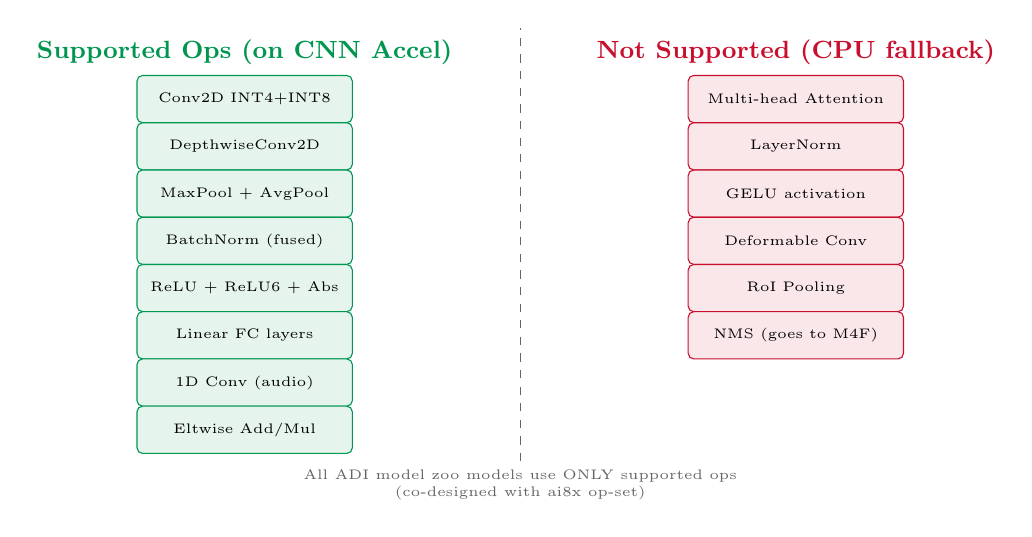
\begin{tikzpicture}[
  opblk/.style={draw=AccentGreen,fill=AccentGreen!10,rounded corners=2pt,
                minimum height=0.6cm,text width=2.5cm,align=center,font=\tiny},
  nopblk/.style={draw=ADIRed,fill=ADIRed!10,rounded corners=2pt,
                 minimum height=0.6cm,text width=2.5cm,align=center,font=\tiny},
]
\node[font=\small\bfseries,text=AccentGreen] at (3.5,5.2) {Supported Ops (on CNN Accel)};
\node[font=\small\bfseries,text=ADIRed] at (10.5,5.2) {Not Supported (CPU fallback)};
\foreach \y/\op in {4.6/{Conv2D INT4+INT8}, 4.0/DepthwiseConv2D, 3.4/{MaxPool + AvgPool},
                     2.8/{BatchNorm (fused)}, 2.2/{ReLU + ReLU6 + Abs},
                     1.6/{Linear FC layers}, 1.0/{1D Conv (audio)}, 0.4/{Eltwise Add/Mul}}
  \node[opblk] at (3.5,\y) {\op};
\foreach \y/\op in {4.6/{Multi-head Attention}, 4.0/LayerNorm, 3.4/{GELU activation},
                     2.8/{Deformable Conv}, 2.2/{RoI Pooling}, 1.6/{NMS (goes to M4F)}}
  \node[nopblk] at (10.5,\y) {\op};
\draw[dashed,ADIGray] (7,0) -- (7,5.5);
\node[font=\tiny,text=ADIGray,align=center] at (7,-0.3)
  {All ADI model zoo models use ONLY supported ops\\(co-designed with ai8x op-set)};
\end{tikzpicture}
\end{frame}

\begin{frame}{5 MB CNN SRAM Fit: Every Model Budget}
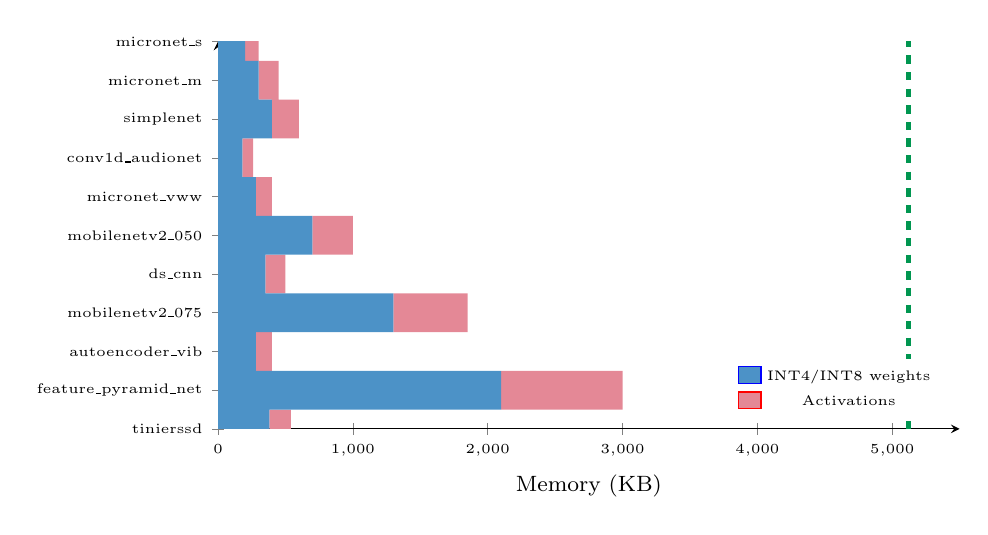
\begin{tikzpicture}
\begin{axis}[
  xbar stacked,
  width=11cm,height=6.5cm,
  bar width=14pt,
  xlabel={\footnotesize Memory (KB)},
  ytick=data,
  yticklabels={micronet\_s,micronet\_m,simplenet,conv1d\_audionet,micronet\_vww,
               mobilenetv2\_050,ds\_cnn,mobilenetv2\_075,autoencoder\_vib,
               feature\_pyramid\_net,tinierssd},
  yticklabel style={font=\tiny},
  xticklabel style={font=\tiny},
  xlabel style={font=\tiny},
  legend style={font=\tiny,at={(0.98,0.02)},anchor=south east,draw=none},
  xmin=0,xmax=5500,
  tick align=inside,axis lines=left,
]
\addplot+[xbar,fill=ADIBlue!70,draw=none]
  coordinates {(200,10)(300,9)(400,8)(180,7)(280,6)
               (700,5)(350,4)(1300,3)(280,2)(2100,1)(380,0)};
\addplot+[xbar,fill=ADIRed!50,draw=none]
  coordinates {(100,10)(150,9)(200,8)(80,7)(120,6)
               (300,5)(150,4)(550,3)(120,2)(900,1)(160,0)};
\addlegendentry{INT4/INT8 weights}
\addlegendentry{Activations}
\draw[dashed,AccentGreen,line width=1.5pt] (axis cs:5120,10.5) -- (axis cs:5120,-0.5)
  node[below,font=\tiny,text=AccentGreen]{5 MB limit};
\end{axis}
\end{tikzpicture}
\end{frame}

\begin{frame}{Model Zoo Design Principles for MAX78002}
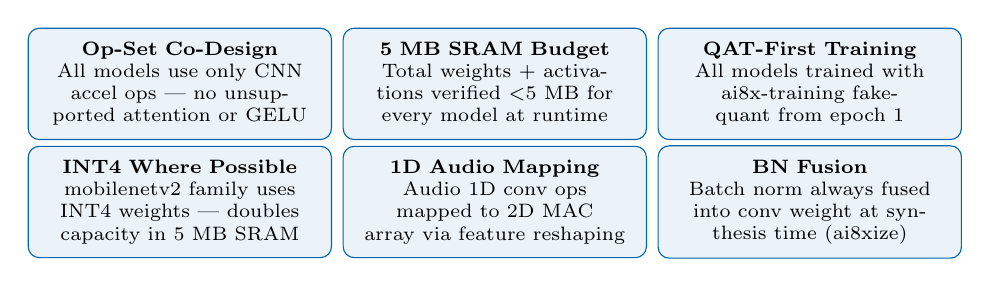
\begin{tikzpicture}[
  principle/.style={draw=ADIBlue,fill=ADIBlue!8,rounded corners=4pt,
                    minimum height=1.3cm,text width=3.5cm,align=center,
                    font=\scriptsize,inner sep=5pt},
]
\node[principle] (p1) at (0,2.5) {\textbf{Op-Set Co-Design}\\All models use only CNN accel ops --- no unsupported attention or GELU};
\node[principle] (p2) at (4.0,2.5) {\textbf{5 MB SRAM Budget}\\Total weights + activations verified $<$5 MB for every model at runtime};
\node[principle] (p3) at (8.0,2.5) {\textbf{QAT-First Training}\\All models trained with ai8x-training fake-quant from epoch 1};
\node[principle] (p4) at (0,1.0) {\textbf{INT4 Where Possible}\\mobilenetv2 family uses INT4 weights --- doubles capacity in 5 MB SRAM};
\node[principle] (p5) at (4.0,1.0) {\textbf{1D Audio Mapping}\\Audio 1D conv ops mapped to 2D MAC array via feature reshaping};
\node[principle] (p6) at (8.0,1.0) {\textbf{BN Fusion}\\Batch norm always fused into conv weight at synthesis time (ai8xize)};
\end{tikzpicture}
\end{frame}

\section{Power Efficiency}

\begin{frame}{Power Consumption: Inference Energy per Frame}
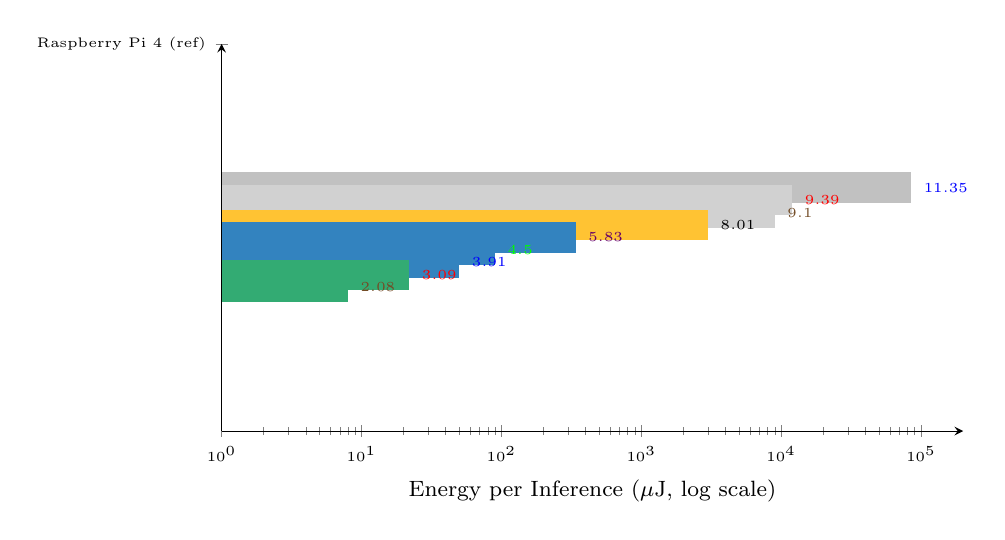
\begin{tikzpicture}
\begin{axis}[
  xbar,
  width=11cm,height=6.5cm,
  bar width=11pt,
  xlabel={\footnotesize Energy per Inference ($\mu$J, log scale)},
  ytick=data,
  yticklabels={
    {Raspberry Pi 4 (ref)},
    {i.MX 8M Plus NPU (NXP)},
    {AM68A NPU (TI)},
    {ADSP-SC835 (ADI audio)},
    {MAX78002 FPN detection},
    {MAX78002 mobilenetv2},
    {MAX78002 simplenet},
    {MAX32690 ds\_cnn},
    {MAX32690 micronet\_s}
  },
  yticklabel style={font=\tiny},
  xticklabel style={font=\tiny},
  xmin=1,xmax=200000,
  tick align=inside,axis lines=left,
  nodes near coords,
  nodes near coords style={font=\tiny,xshift=1pt},
  xmode=log,
]
\addplot+[xbar,fill=ADIGray!40,draw=none] coordinates {(85000,8)};
\addplot+[xbar,fill=ADIGray!30,draw=none] coordinates {(12000,7)};
\addplot+[xbar,fill=ADIGray!30,draw=none] coordinates {(9000,6)};
\addplot+[xbar,fill=ADIGold!80,draw=none] coordinates {(3000,5)};
\addplot+[xbar,fill=ADIBlue!80,draw=none] coordinates {(340,4)};
\addplot+[xbar,fill=ADIBlue!80,draw=none] coordinates {(90,3)};
\addplot+[xbar,fill=ADIBlue!80,draw=none] coordinates {(50,2)};
\addplot+[xbar,fill=AccentGreen!80,draw=none] coordinates {(22,1)};
\addplot+[xbar,fill=AccentGreen!80,draw=none] coordinates {(8,0)};
\end{axis}
\end{tikzpicture}
\end{frame}

\begin{frame}{Battery Life Estimation: MAX32690 KWS Application}
\begin{columns}
\column{0.55\textwidth}
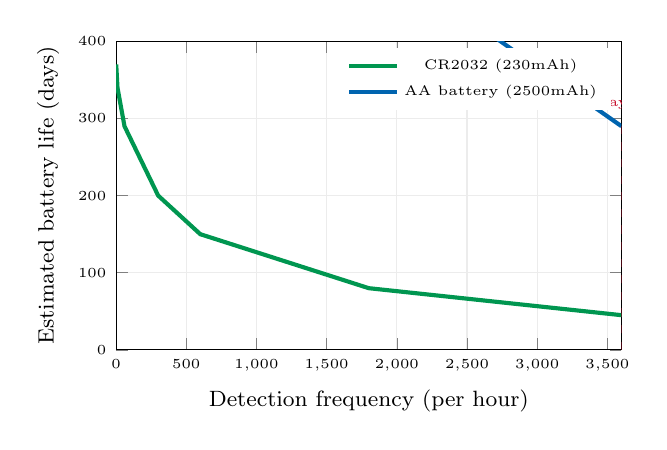
\begin{tikzpicture}
\begin{axis}[
  width=8cm,height=5.5cm,
  xlabel={\footnotesize Detection frequency (per hour)},
  ylabel={\footnotesize Estimated battery life (days)},
  xmin=0,xmax=3600,
  ymin=0,ymax=400,
  grid=major,grid style={gray!15},
  legend style={font=\tiny,at={(0.98,0.98)},anchor=north east,draw=none},
  xlabel style={font=\tiny},
  ylabel style={font=\tiny},
  xticklabel style={font=\tiny},
  yticklabel style={font=\tiny},
]
\addplot+[line width=1.5pt,color=AccentGreen,no marks]
  coordinates {(1,370)(10,340)(60,290)(300,200)(600,150)(1800,80)(3600,45)};
\addlegendentry{CR2032 (230mAh)}
\addplot+[line width=1.5pt,color=ADIBlue,no marks]
  coordinates {(1,2500)(10,2300)(60,1900)(300,1300)(600,950)(1800,520)(3600,290)};
\addlegendentry{AA battery (2500mAh)}
\draw[dashed,ADIRed] (axis cs:3600,0) -- (axis cs:3600,300)
  node[above,font=\tiny,text=ADIRed]{always-on};
\end{axis}
\end{tikzpicture}
\column{0.42\textwidth}
\footnotesize
\begin{block}{KWS Power Budget}
\begin{itemize}
  \item Sleep: $<$10 $\mu$A
  \item Inference (120ms burst): $\sim$2 mA
  \item Average (1/hour): $\sim$0.3 mA
\end{itemize}
\end{block}
\begin{block}{Practical Example}
Smart home sensor: keyword once per minute. AA battery $\rightarrow$ \textbf{$>$1.5 years}. CR2032 $\rightarrow$ \textbf{$>$9 months}.
\end{block}
\begin{alertblock}{Competitors need plug}
\footnotesize Most Cortex-A IoT devices require wall power. MAX32690 runs \textbf{years} on a battery.
\end{alertblock}
\end{columns}
\end{frame}

\section{Multi-Model Pipelines}

\begin{frame}{Smart Sensor Node: Hierarchical Activation Pipeline}
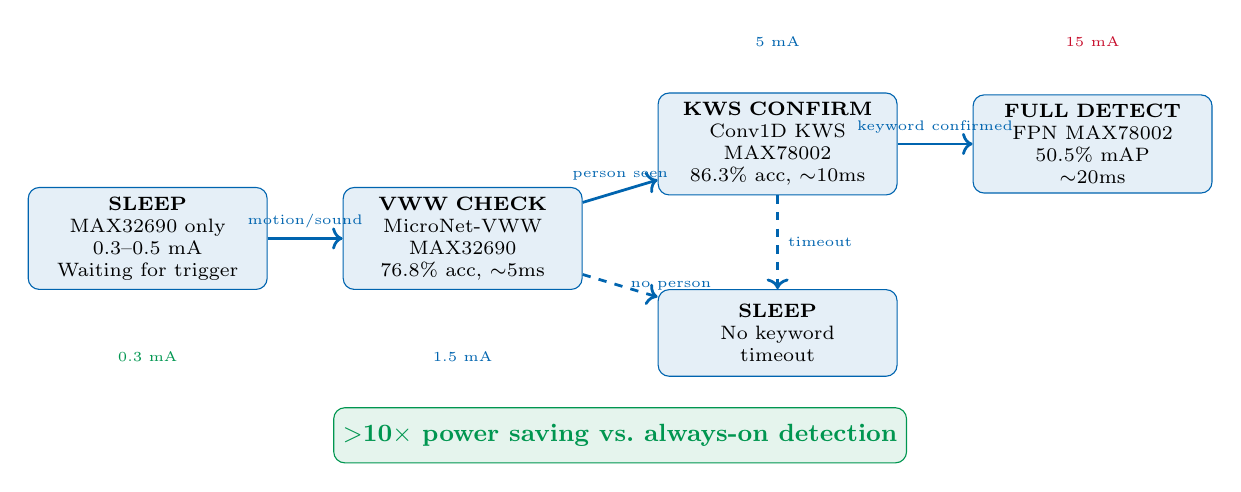
\begin{tikzpicture}[
  sbox/.style={draw=ADIBlue,fill=ADIBlue!10,rounded corners=4pt,
               minimum height=1.1cm,text width=2.8cm,align=center,font=\scriptsize},
]
\node[sbox] (sleep) at (0,0) {\textbf{SLEEP}\\MAX32690 only\\0.3--0.5 mA\\Waiting for trigger};
\node[sbox] (vww) at (4.0,0) {\textbf{VWW CHECK}\\MicroNet-VWW\\MAX32690\\76.8\% acc, $\sim$5ms};
\node[sbox] (kws) at (8.0,1.2) {\textbf{KWS CONFIRM}\\Conv1D KWS\\MAX78002\\86.3\% acc, $\sim$10ms};
\node[sbox] (det) at (12.0,1.2) {\textbf{FULL DETECT}\\FPN MAX78002\\50.5\% mAP\\$\sim$20ms};
\node[sbox] (reject) at (8.0,-1.2) {\textbf{SLEEP}\\No keyword\\timeout};
\draw[->,ADIBlue,line width=1pt] (sleep) -- (vww)
  node[midway,above,font=\tiny]{motion/sound};
\draw[->,ADIBlue,line width=1pt] (vww) -- (kws)
  node[midway,above,font=\tiny]{person seen};
\draw[->,ADIBlue,line width=1pt] (kws) -- (det)
  node[midway,above,font=\tiny]{keyword confirmed};
\draw[->,ADIBlue,dashed,line width=1pt] (vww) -- (reject)
  node[midway,right,font=\tiny]{no person};
\draw[->,ADIBlue,dashed,line width=1pt] (kws) -- (reject)
  node[midway,right,font=\tiny]{timeout};
\node[font=\tiny,text=AccentGreen] at (0,-1.5) {0.3 mA};
\node[font=\tiny,text=ADIBlue] at (4.0,-1.5) {1.5 mA};
\node[font=\tiny,text=ADIBlue] at (8.0,2.5) {5 mA};
\node[font=\tiny,text=ADIRed] at (12.0,2.5) {15 mA};
\node[draw=AccentGreen,fill=AccentGreen!10,rounded corners,font=\small\bfseries,
      text=AccentGreen,minimum width=4cm,minimum height=0.7cm]
  at (6,-2.5) {$>$10$\times$ power saving vs.\ always-on detection};
\end{tikzpicture}
\end{frame}

\begin{frame}{Predictive Maintenance Pipeline: Vibration + Vision}
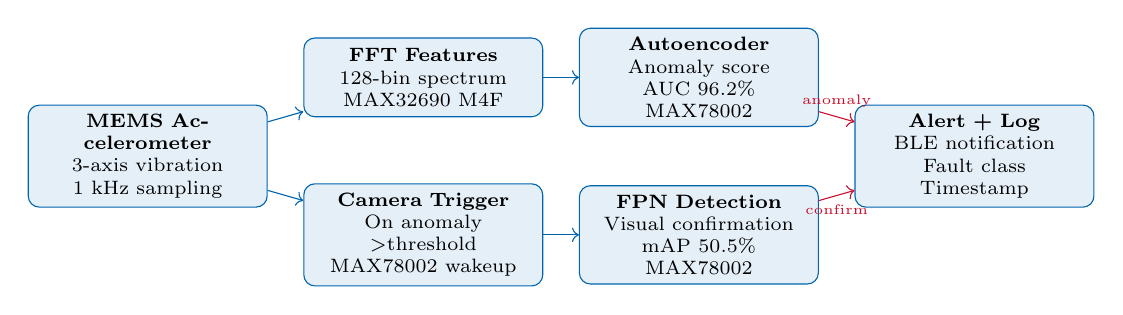
\begin{tikzpicture}[
  mbox/.style={draw=ADIBlue,fill=ADIBlue!10,rounded corners=4pt,
               minimum height=1.0cm,text width=2.8cm,align=center,font=\scriptsize},
]
\node[mbox] (accel) at (0,1.5) {\textbf{MEMS Accelerometer}\\3-axis vibration\\1 kHz sampling};
\node[mbox] (fft) at (3.5,2.5) {\textbf{FFT Features}\\128-bin spectrum\\MAX32690 M4F};
\node[mbox] (ae) at (7.0,2.5) {\textbf{Autoencoder}\\Anomaly score\\AUC 96.2\%\\MAX78002};
\node[mbox] (cam) at (3.5,0.5) {\textbf{Camera Trigger}\\On anomaly $>$threshold\\MAX78002 wakeup};
\node[mbox] (fpn) at (7.0,0.5) {\textbf{FPN Detection}\\Visual confirmation\\mAP 50.5\%\\MAX78002};
\node[mbox] (alert) at (10.5,1.5) {\textbf{Alert + Log}\\BLE notification\\Fault class\\Timestamp};
\draw[->,ADIBlue] (accel) -- (fft);
\draw[->,ADIBlue] (fft) -- (ae);
\draw[->,ADIBlue] (accel) -- (cam);
\draw[->,ADIBlue] (cam) -- (fpn);
\draw[->,ADIRed] (ae) -- (alert) node[midway,above,font=\tiny]{anomaly};
\draw[->,ADIRed] (fpn) -- (alert) node[midway,below,font=\tiny]{confirm};
\end{tikzpicture}
\end{frame}

\section{Development Ecosystem}

\begin{frame}{ADI AI8X Development Ecosystem}
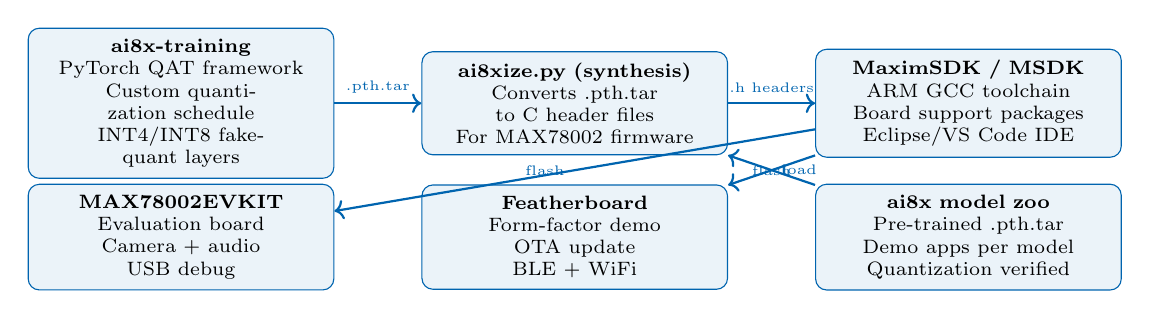
\begin{tikzpicture}[
  tool/.style={draw=ADIBlue,fill=ADIBlue!8,rounded corners=4pt,
               minimum width=3.8cm,minimum height=1.1cm,
               text width=3.6cm,align=center,font=\scriptsize,inner sep=4pt},
]
\node[tool] (aitrain) at (0,3.5) {\textbf{ai8x-training}\\PyTorch QAT framework\\Custom quantization schedule\\INT4/INT8 fake-quant layers};
\node[tool] (aisynth) at (5.0,3.5) {\textbf{ai8xize.py (synthesis)}\\Converts .pth.tar\\to C header files\\For MAX78002 firmware};
\node[tool] (msdk) at (10.0,3.5) {\textbf{MaximSDK / MSDK}\\ARM GCC toolchain\\Board support packages\\Eclipse/VS Code IDE};
\node[tool] (evkit) at (0,1.8) {\textbf{MAX78002EVKIT}\\Evaluation board\\Camera + audio\\USB debug};
\node[tool] (fthr) at (5.0,1.8) {\textbf{Featherboard}\\Form-factor demo\\OTA update\\BLE + WiFi};
\node[tool] (modelzoo) at (10.0,1.8) {\textbf{ai8x model zoo}\\Pre-trained .pth.tar\\Demo apps per model\\Quantization verified};
\draw[->,ADIBlue,line width=0.8pt] (aitrain) -- (aisynth)
  node[midway,above,font=\tiny]{.pth.tar};
\draw[->,ADIBlue,line width=0.8pt] (aisynth) -- (msdk)
  node[midway,above,font=\tiny]{.h headers};
\draw[->,ADIBlue,line width=0.8pt] (msdk) -- (evkit)
  node[midway,left,font=\tiny]{flash};
\draw[->,ADIBlue,line width=0.8pt] (msdk) -- (fthr)
  node[midway,font=\tiny]{flash};
\draw[->,ADIBlue,line width=0.8pt] (modelzoo) -- (aisynth)
  node[midway,right,font=\tiny]{load};
\end{tikzpicture}
\end{frame}

\begin{frame}{MLOps Pipeline for ADI AI8X}
\small
\begin{tabular}{llll}
\toprule
\textbf{Stage} & \textbf{Tool} & \textbf{Artifact} & \textbf{Gate}\\
\midrule
Experiment tracking & MLflow & run metrics, QAT params & ---\\
QAT training & ai8x-training + Optuna HPO & .pth.tar & Acc drop $<$0.5\%\\
Synthesis & ai8xize.py & C header files & Synthesis succeeds\\
Model registry & MLflow Registry & Staging $\rightarrow$ Production & mAP/KWS $>$ threshold\\
Orchestration & Prefect 2 flows & Train+Synth+Eval DAG & Task-level retries\\
Drift detection & Evidently AI & Accuracy + confidence & $>$5\% drift $\rightarrow$ alert\\
CI/CD & GitHub Actions & 6-job pipeline & All gates pass\\
Infrastructure & AWS CDK v2 (g4dn.xlarge) & S3+ECR+ECS+CW & GPU spot\\
\bottomrule
\end{tabular}
\vspace{0.3cm}
\begin{block}{Optuna HPO Parameters}
\footnotesize Tunes: \texttt{weight\_bits} (4 vs 8), \texttt{lr} (1e-4--1e-2), \texttt{batch\_size} (32--128), \texttt{qat\_start\_epoch} (10--30), \texttt{weight\_decay}. Objective: maximize accuracy + minimize model memory.
\end{block}
\end{frame}

\begin{frame}{Summary: ADI AI8X at a Glance}
\begin{columns}
\column{0.55\textwidth}
\small
\begin{tabular}{lcc}
\toprule
\textbf{Dimension} & \textbf{Score} & \textbf{Notes}\\
\midrule
Power efficiency & $\bigstar\bigstar\bigstar\bigstar\bigstar$ & 0.3--15 mA\\
Quantization quality & $\bigstar\bigstar\bigstar\bigstar\bigstar$ & QAT $<$0.5\% drop\\
Battery life & $\bigstar\bigstar\bigstar\bigstar\bigstar$ & Years on coin cell\\
Energy per inference & $\bigstar\bigstar\bigstar\bigstar\bigstar$ & 8--340 $\mu$J\\
Model variety & $\bigstar\bigstar\bigstar$ & 15 models, 6 tasks\\
Peak accuracy & $\bigstar\bigstar\bigstar$ & Op-set limits arch\\
Audio support & $\bigstar\bigstar\bigstar\bigstar$ & KWS+denoise+genre\\
Multi-model pipeline & $\bigstar\bigstar\bigstar\bigstar$ & Hierarchical power mgmt\\
Dev.\ ecosystem & $\bigstar\bigstar\bigstar\bigstar$ & ai8x SDK mature\\
\bottomrule
\end{tabular}
\column{0.42\textwidth}
\begin{block}{Key Differentiators}
\begin{itemize}
  \item \textbf{442 TOPS/W} --- unmatched power efficiency
  \item \textbf{QAT}: INT4 weights possible, near-zero accuracy loss
  \item \textbf{5 MB on-chip SRAM}: no external DDR during inference
  \item \textbf{Multi-modal}: vision + audio + vibration in one node
  \item \textbf{Hierarchical activation}: $>$10$\times$ power saving
\end{itemize}
\end{block}
\begin{alertblock}{Best Fit When\ldots}
\footnotesize Battery-powered IoT, wearable, or smart sensor where power is the \#1 constraint --- not peak accuracy or model variety.
\end{alertblock}
\end{columns}
\end{frame}

\end{document}
